% Copyright (C) 2005-2015 Airbus - EDF - IMACS - Phimeca
% Permission is granted to copy, distribute and/or modify this document
% under the terms of the GNU Free Documentation License, Version 1.2
% or any later version published by the Free Software Foundation;
% with no Invariant Sections, no Front-Cover Texts, and no Back-Cover
% Texts.  A copy of the license is included in the section entitled "GNU
% Free Documentation License".
\renewcommand{\filename}{docUC_InputNoData_ProductDistribution.tex}
\renewcommand{\filetitle}{UC : Creation  of 1D distribution as the product of 1D distributions}

% \HeaderNNIILevel
% \HeaderIILevel
\HeaderIIILevel

\index{Product Distribution}

The objective of the Use Case is to create a distribution, defined as the prodcut of univariate distributions.\\

If we note $\mathcal{L}_X$ and $\mathcal{L}_Y$ two univariate distributions, OpenTURNS enables to easily create the distribution  $\mathcal{L}$ of the random variable $Z$ defined by:
\begin{align}
  Z=XY
\end{align}
where $(X,Y)$ are independent with respective marginal distributions  $\mathcal{L}_X$ and $\mathcal{L}_Y$.

\textspace\\

\noindent%
\requirements{
  \begin{description}
  \item[$\bullet$] two independent  univariate distribution : {\itshape distX, distY}
  \item[type:] Distribution
  \end{description}
}
{
  \begin{description}
  \item[$\bullet$] the product distribution : {\itshape distZ}
  \item[type:] ProductDistribution
  \end{description}
}

\textspace\\
Python script for this UseCase :

\inputscript{script_docUC_InputNoData_ProductDistribution}

\textspace\\

The figure \ref{prodDist} illustrates the product distribution where:
\begin{itemize}
\item  $\mathcal{L}_X = Uniform(0, 1)$,
\item  $\mathcal{L}_Y = Uniform(2, 3)$.
\end{itemize}




\begin{figure}[H]
  \begin{center}
    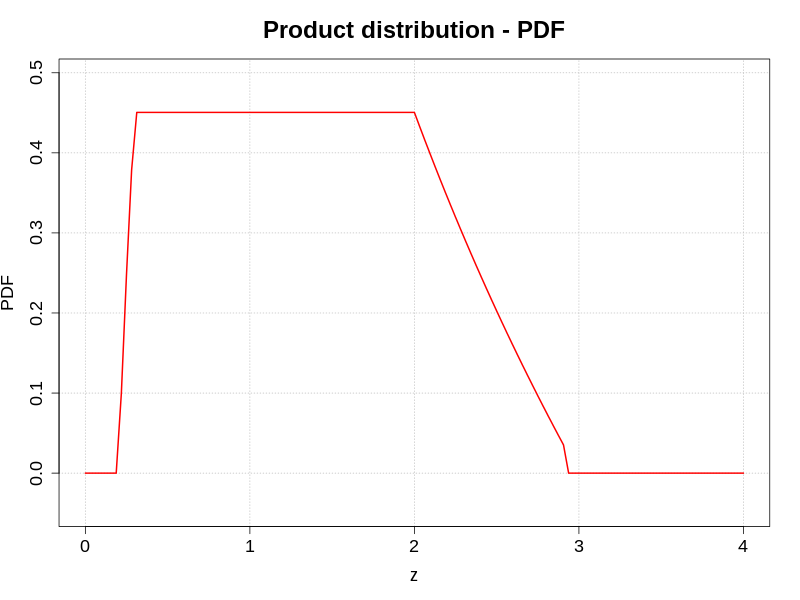
\includegraphics[width=7cm]{Figures/productDist.png}
    \caption{PDF $Z=XY$ where $(X, Y)$ are independent with respective marginal distributions $Uniform(0, 1$) and $Uniform(2, 3)$.}
    \label{prodDist}
  \end{center}
\end{figure}
